\documentclass[11pt,fleqn]{article} 
\usepackage[margin=0.8in, head=0.8in]{geometry} 
\usepackage{amsmath, amssymb, amsthm}
\usepackage{fancyhdr} 
\usepackage{palatino, url, multicol}
\usepackage{graphicx} 
\usepackage[all]{xy}
\usepackage{polynom} 
%\usepackage{pdfsync}
\usepackage{enumerate}
\usepackage{framed}
\usepackage{setspace}
\usepackage{array,tikz,pgfplots}

% TiKZ.
\usepackage{tikz, pgfplots}
\usetikzlibrary{calc}
\pgfplotsset{my style/.append style={axis x line=middle, axis y line=
middle, xlabel={$x$}, ylabel={$y$}, axis equal }}

\pgfplotsset{compat=1.6}

\pgfplotsset{soldot/.style={color=black,only marks,mark=*}} \pgfplotsset{holdot/.style={color=black,fill=white,only marks,mark=*}}

\pagestyle{fancy} 
\lfoot{UAF Calculus 1}
\rfoot{2-7}

\begin{document}
\setlength{\parindent}{0cm}
\renewcommand{\headrulewidth}{0pt}
\newcommand{\blank}[1]{\rule{#1}{0.75pt}}
\renewcommand{\d}{\displaystyle}
\vspace*{-0.9in}
\begin{center}
  \Large \sc{Section 2-8}
\end{center}
\small
\begin{enumerate}
\item  For each problem below, you are given the graph of $f(x)$. You must sketch the graph of $f'(x)$ on the axes below.

\begin{tabular}{cc}
%quadratic
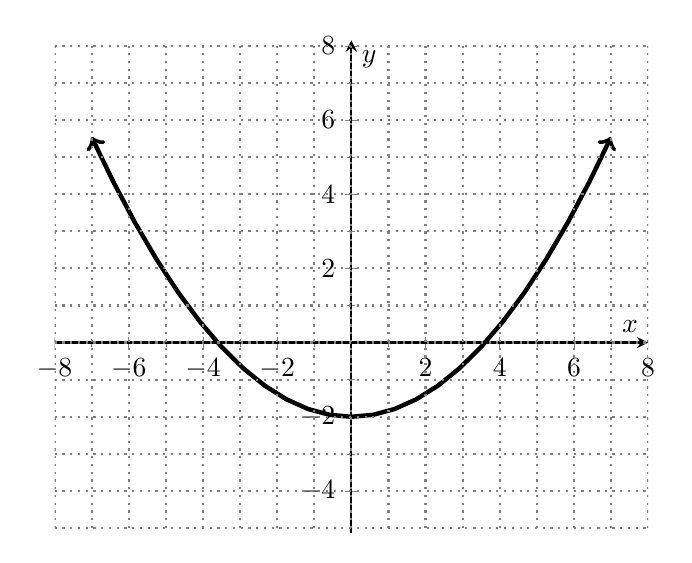
\begin{tikzpicture}
\begin{axis}[scale=1.1, thick, my style, xtick={-8,-6,...,8}, ytick={-4,-2,...,8},
xmin=-8, xmax=8, ymin=-5, ymax=8, minor y tick num=1,
        minor x tick num=1, mark size=3.0pt]
        \addplot[ultra thick, <->,domain=-7:7]{x*x/6.5 -2};
\foreach \i in {-8,-7,-6,...,8}{
	\addplot[dotted, gray, domain=-8:8]{\i};
	\addplot[dotted, gray] coordinates {(\i,-5) (\i,8)};
	}
\end{axis}
\end{tikzpicture}

&
%linear
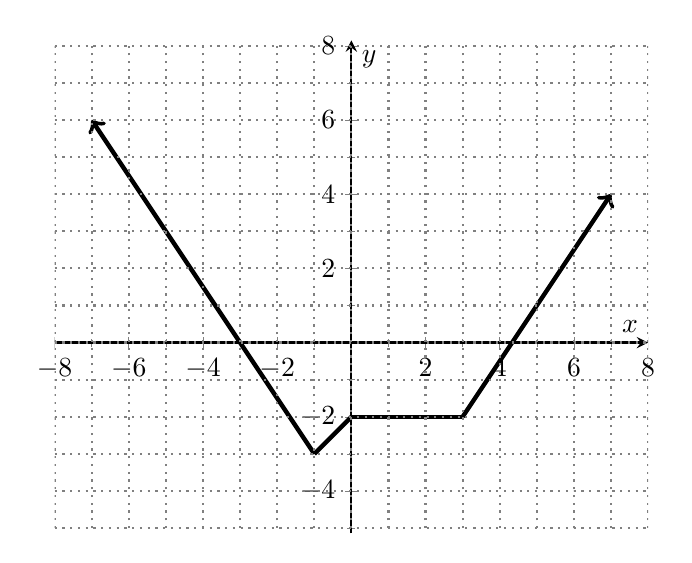
\begin{tikzpicture}
\begin{axis}[scale=1.1, thick, my style, xtick={-8,-6,...,8}, ytick={-8,-6,...,8},
xmin=-8, xmax=8, ymin=-5, ymax=8, minor y tick num=1,
        minor x tick num=1, mark size=3.0pt]
\addplot[ultra thick, smooth,<-] coordinates {(-7,6) (-1,-3)};
\addplot[ultra thick, smooth] coordinates {(-1,-3) (0,-2)};
\addplot[ultra thick, smooth] coordinates {(0,-2) (3,-2)};
\addplot[ultra thick, smooth,->] coordinates {(3,-2) (7,4)};
\foreach \i in {-8,-7,-6,...,8}{
	\addplot[dotted, gray, domain=-8:8]{\i};
	\addplot[dotted, gray] coordinates {(\i,-5) (\i,8)};
	}
\end{axis}
\end{tikzpicture}
\\
\end{tabular}

%%%%SAMPLE
%%%%%%%%%%
\begin{tabular}{cc}
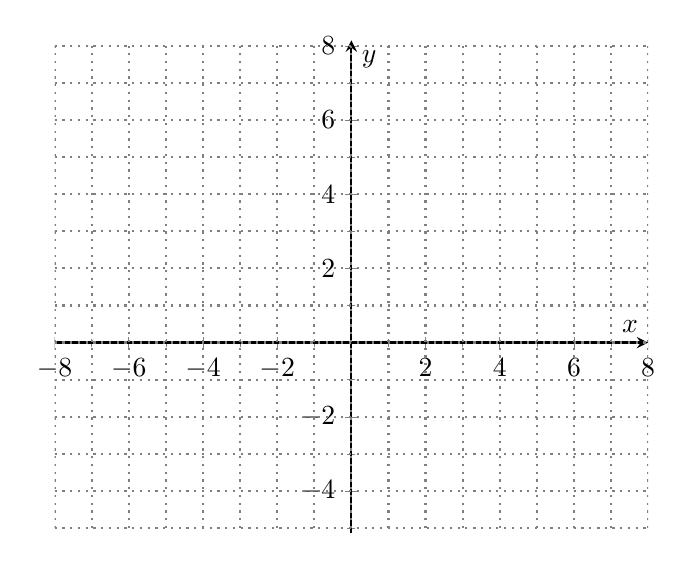
\begin{tikzpicture}
\begin{axis}[scale=1.1, thick, my style, xtick={-8,-6,...,8},ytick={-8,-6,...,8}, xmin=-8, xmax=8, ymin=-5, ymax=8, minor y tick num=1,
        minor x tick num=1, mark size=3.0pt]
\foreach \i in {-8,-7,-6,...,8}{
	\addplot[dotted, gray, domain=-8:8]{\i};
	\addplot[dotted, gray] coordinates {(\i,-5) (\i,8)};
	}
\end{axis}
\end{tikzpicture}

&
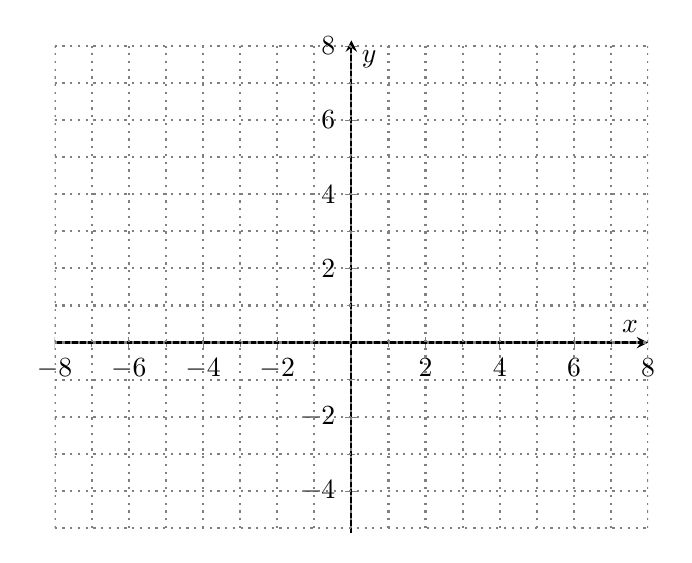
\begin{tikzpicture}
\begin{axis}[scale=1.1, thick, my style, xtick={-8,-6,...,8}, ytick={-4,-2,...,8},
xmin=-8, xmax=8, ymin=-5, ymax=8, minor y tick num=1,
        minor x tick num=1, mark size=3.0pt]
\foreach \i in {-8,-7,-6,...,8}{
	\addplot[dotted, gray, domain=-8:8]{\i};
	\addplot[dotted, gray] coordinates {(\i,-5) (\i,8)};
	}
\end{axis}
\end{tikzpicture}
\\
\end{tabular}

\item For each problem below, make your own sketch of $f(x)$ and use it to sketch $f'(x).$
	\begin{enumerate}
	\item $f(x)=|x|$
	\vfill
	\item $f(x)=\ln x$
	\vfill
	\end{enumerate}
\newpage
\item The derivative of  $f(x)=x^{1/3}$ is $f'(x)=\frac{1}{3x^{2/3}}.$ Explain why $f$ does not have a derivative at $x=0$ but it does have a tangent line at $x=0.$
\vfill

\item For the functions in parts 1 and 2, draw $f''(x)$, the derivative of the derivative (or the second derivative).
\vfill 
\end{enumerate}
 \end{document}